\documentclass[10pt,a4paper]{article}
 
\usepackage{etex} % расширение классического tex в частности позволяет подгружать гораздо больше пакетов, чем мы и займёмся далее
 
%%%%%%%%%% Математика %%%%%%%%%%
\usepackage{amsmath,amsfonts,amssymb,amsthm,mathtools}
%\mathtoolsset{showonlyrefs=true}  % Показывать номера только у тех формул, на которые есть \eqref{} в тексте.
%\usepackage{leqno} % Нумерация формул слева
 
 
%%%%%%%%%%%%%%%%%%%%%%%% Шрифты %%%%%%%%%%%%%%%%%%%%%%%%%%%%%%%%%
 
\usepackage{fontspec}         % пакет для подгрузки шрифтов
\setmainfont{Arial}   % задаёт основной шрифт документа
 
\defaultfontfeatures{Mapping=tex-text}
 
% why do we need \newfontfamily:
% http://tex.stackexchange.com/questions/91507/
\newfontfamily{\cyrillicfonttt}{Arial}
\newfontfamily{\cyrillicfont}{Arial}
\newfontfamily{\cyrillicfontsf}{Arial}
 
\usepackage{unicode-math}     % пакет для установки математического шрифта
\setmathfont{Asana Math}      % шрифт для математики
 
\usepackage{polyglossia}      % Пакет, который позволяет подгружать русские буквы
\setdefaultlanguage{russian}  % Основной язык документа
\setotherlanguage{english}    % Второстепенный язык документа
 
 
 
%%%%%%%%%% Работа с картинками %%%%%%%%%
\usepackage{graphicx}                  % Для вставки рисунков
\usepackage{graphics}
\graphicspath{{images/}{pictures/}}    % можно указать папки с картинками
\usepackage{wrapfig}                   % Обтекание рисунков и таблиц текстом
\usepackage{subfigure}                 % для создания нескольких рисунков внутри одного
 
 
%%%%%%%%%% Работа с таблицами %%%%%%%%%%
\usepackage{tabularx}            % новые типы колонок
\usepackage{tabulary}            % и ещё новые типы колонок
\usepackage{array}               % Дополнительная работа с таблицами
\usepackage{longtable}           % Длинные таблицы
\usepackage{multirow}            % Слияние строк в таблице
\usepackage{float}               % возможность позиционировать объекты в нужном месте
\usepackage{booktabs}            % таблицы как в книгах!
\renewcommand{\arraystretch}{1.3} % больше расстояние между строками
 
 
 
 
\DeclareMathOperator{\diag}{diag}  % математический оператор, который описывает диагональную матрицу
 
\usepackage[landscape,top=2mm, bottom=2mm,left=2mm,right=2mm,includefoot]{geometry}
 
 
 
\begin{document}
\pagestyle{empty}
 
 
\begin{table}[h!]
\begin{center}
\scalebox{0.91}{
\footnotesize
\begin{tabular}{| p{0.13\linewidth} | p{0.18\linewidth}| p{0.07\linewidth} | p{0.1\linewidth} |p{0.12\linewidth} |p{0.4\linewidth} |}
\hline
 
\begin{center}Метод \end{center}&\begin{center} Оценка \end{center} & \begin{center}Год создания \end{center}& \begin{center}Автор \end{center} & \begin{center}Фотка автора \end{center} & \begin{center}Описание \end{center}\\
\hline
\begin{center} Метод наименьших квадратов \newline (OLS) \end{center} & \begin{center}  \[ (X^{T}X)^{-1}X^Ty \]\end{center} & \begin{center}1795 \end{center}& \begin{center} Carl Friedrich Gauss \newline Лежандр \end{center} &  \center{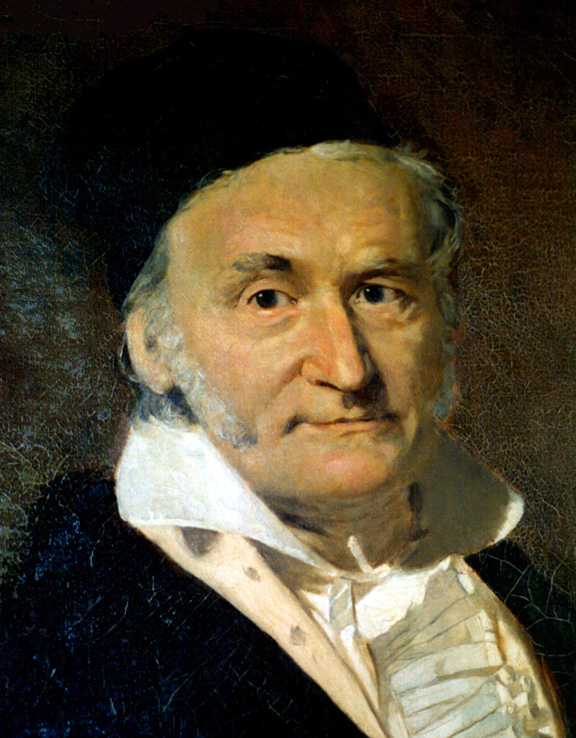
\includegraphics[width=0.4\linewidth]{gauss.jpg}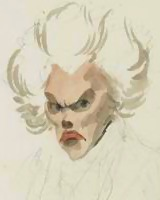
\includegraphics[width=0.41\linewidth]{lezhandr.jpg}    }  &\begin{center} Метод оценивания параметров эконометрической модели, состоящий в минимизации суммы квадратов расхождений между наблюдаемыми значениями зависимой переменной и значениями этой переменной, вычисленными для наблюдаемых значений независимых переменных по оценённой модели связи. \end{center}\\
\hline
\begin{center}Обобщённый метод наименьших квадратов \newline(GLS) \end{center} &\begin{center} \[(X^T \Omega^{-1} X)^{-1}X^T \Omega^{-1} y\]\end{center} & \begin{center}1934 \end{center}& \begin {center}Alexander Aitken \end{center} & \begin{center}не нашёл \end{center} & \begin{center}Теоретическая процедура оценивания коэффициентов линенйиной модели регрессии в ситуации, когда случайные ошибки имеют разные дисперсии и коррелированы между собой, при этом предполагается,  что ковариационная матрица вектора ошибок невырождена и все ее элементы известны. \end{center} \\
\hline
\begin{center}Взвешенный метод наименьших квадратов \newline (WLS) \end{center}& \begin{center} $\begin{aligned}  &(X^T \Omega^{-1} X)^{-1}  X^T \Omega^{-1} y \\ &\text{ при этом } \\ &\Omega = \diag(\sigma_1,\sigma_2, \ldots \sigma_n) 
\end{aligned}$\end{center}&\begin{center}  он же \end{center} & \begin{center}он же \end{center}& \begin{center}не нашел \end{center}  & \begin{center}Процедура, состоящая в минимизации определённым образом взвешенной суммы квадратов отклонений наблюдаемых значений зависиммой переменной от значений, вычисляемых по подбираемой модели связи. \end{center}\\
\hline
\begin{center}Доступный обобщённый метод наименьших квадратов \newline (FGLS)\end{center} & \begin{center} \[(X^T \hat{\Omega}^{-1} X)^{-1}X^T \hat{\Omega}^{-1} y\]\end{center}& \begin{center}тот же  \end{center}& \begin{center} он же \end{center} & \begin{center}не нашел  \end{center}& \begin{center}Практически реализуемая процедура оценивания коэффициентов линейной модели регрессии в ситуации, когда случайные ошибки имеют разные дисперсии и коррелированы между собой, повторяющая процедуру обобщенного метода наисеньших квадратов, но импользующая оцененную ковариационную матрицу вектора ошибок.\end{center} \\
\hline
\begin{center}Косвенный метод наименьших квадратов \newline(ILS) \end{center} & & \begin{center} В 1928 начали заниматься проблемой инструментальных переменных\end{center}  & \begin{center} Philip Wright \newline Sewall Wright \newline (отец и сын) \end{center}& \center{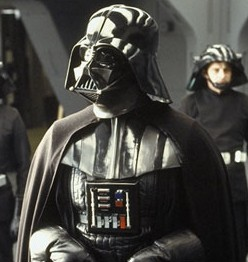
\includegraphics[width=0.52\linewidth]{Darth_Vader.jpg}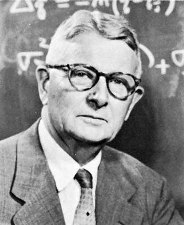
\includegraphics[width=0.45\linewidth]{Sewall_Wright.jpg}}  & \begin{center}Mетод получения оценок параметров $i-$го стохастического уравнения структурной формы через оценки наименьших квадратов коэффициентов уравнений приведенной формы. Метод применим в случае точной идентифицируемости $i-$го структурного уравнения. \end{center}\\
\hline
\begin{center} Двухшаговый метод наименьших квадратов \newline(2SLS) \end{center}& \begin{center}\[(X^T Z (Z^T Z)^{-1} Z^T X)^{-1} X^T Z(Z^T Z)^{-1} Z^Ty \]\end{center}& \begin{center}1953  \newline   1957 \end{center}& \begin{center} Henri Theil \newline Robert Basmann \end{center} &\begin{center} не нашёл \end{center} & \begin{center} Метод оценивания коэффициентов уравнения структурной формы, состоящий в предварительной очистке стохастической объясняющей переменой от коррелированности с ошибкой в этом уравнении с использованием инструментальных переменных и в последующем оценивании уравнения, в котором исходная объясняющая переменная заменяется ее очищенным вариантом. \end{center} \\
\hline
\begin{center}Трёхшаговый метод наименьших квадратов \newline(3SLS) \end{center} & \[ (\hat Z^T(\hat \Lambda^{-1} \otimes I_g) \hat Z)^{-1} \hat Z^T (\hat \Lambda^{-1} \otimes I_g)y \] & \begin{center}они же \end{center} &\begin{center} они же\end{center} & \begin{center}они же \end{center}  & \begin{center}Доступный обобщённый метод наименьших квадратов, применённый к системе одновременных уравнений. Принимает во внимание наличие коррелирванности между ошибками в разных структурных уравнениях. \end{center}\\
\hline
\end{tabular}}
\end{center}
\end{table}
 
\end{document}